\documentclass[11pt]{article}

\input{../../preamble.tex}

\usepackage[margin=1in]{geometry}
\usepackage{amsmath,amssymb,bm}
\usepackage{graphicx}
\usepackage{float}
\usepackage{setspace}
\usepackage{tikz}
\usetikzlibrary{calc}

% ---------- Small helpers ----------
\newcommand{\kb}[1]{\bm{k}_{#1}}
\newcommand{\ob}[1]{\bm{o}_{#1}}
\newcommand{\vb}{\bm{v}}
\newcommand{\wb}{\bm{\omega}}
\newcommand{\J}{\bm{J}}
\newcommand{\q}{\bm{q}}
\newcommand{\qd}{\dot{\bm{q}}}
\newcommand{\twist}{\begin{bmatrix}\vb\\ \wb\end{bmatrix}}

\begin{document}

\begin{center}

{\Large University of British Columbia}

\vspace{0.2cm}

MECH 464/563 EECE 442/589: Introduction to Robotics

\vspace{0.2cm}

{\large Image Processing Homework, due Friday March 6}

\end{center}

\begin{enumerate}
    \item We apply erosion to the white speckled images to expand the black regions over it's white speckles, and dilation to expand the white regions over the black speckles in the black speckled regions.
        The best kernel shape and size is the same for both image types: size 3, shape: circle.

\begin{figure}[htbp]
    \centering
    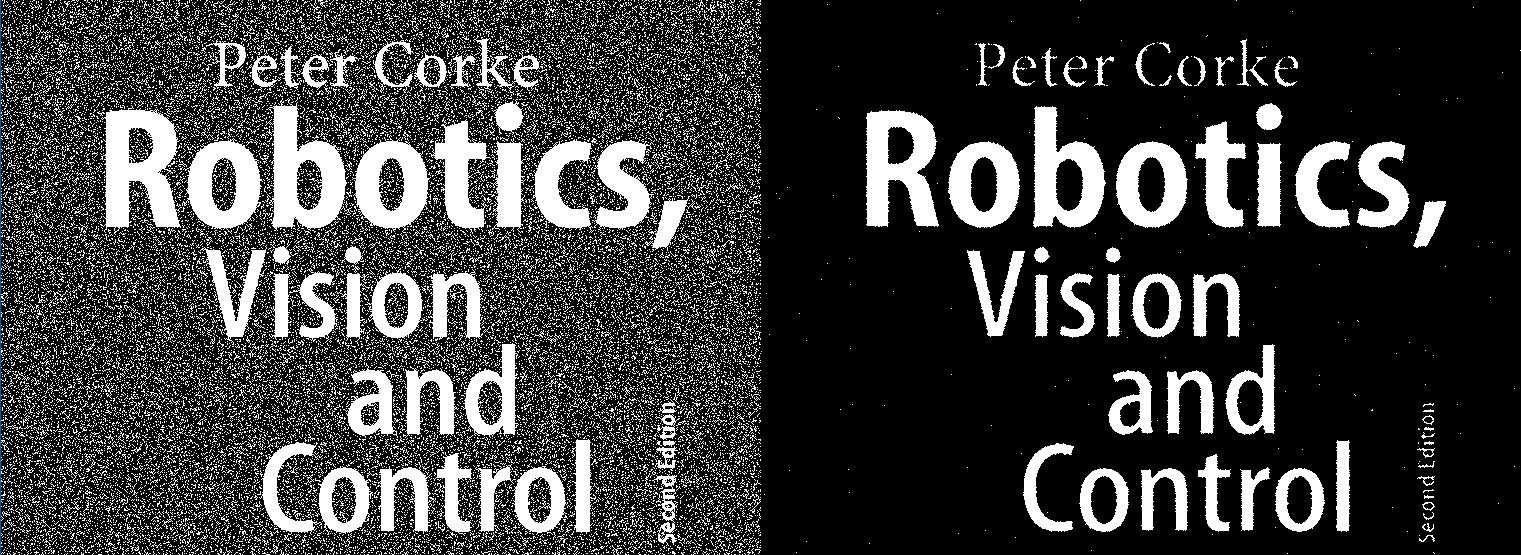
\includegraphics[width=\textwidth]{White_speckled.png}

    \vspace{0.5em} % optional spacing between images

    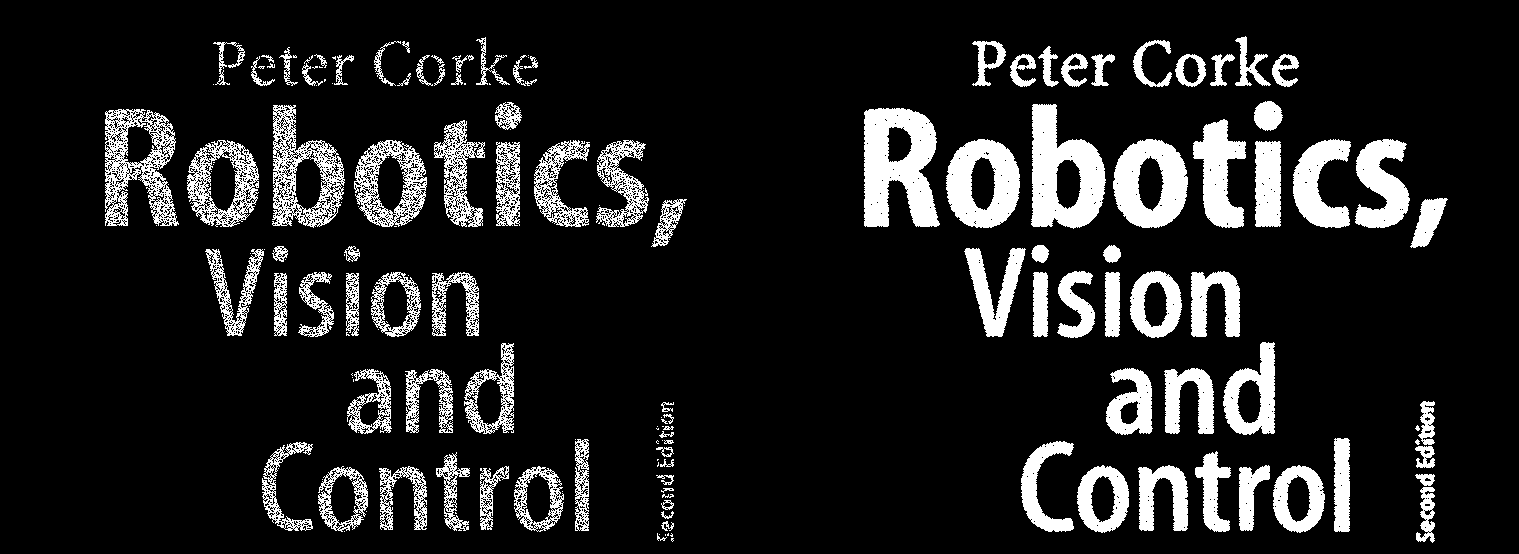
\includegraphics[width=\textwidth]{Black_speckled.png}

    \caption{Best erosion (top) (SSIM 0.8965) and dialation (bottom) (SSIM 0.9039)}
    \label{fig:speckled_patterns}
\end{figure}
\item The region of interest was determined manually by trial and error, to find the rectangle precisely covering the author's name, "Peter Corke".
We have the following program output:
\begin{verbatim}
============================================================
TASK 2: OCR / Character Recognition
============================================================
Author Name: Peter Corke
\end{verbatim}
\item In order to determine the colours of each cluster in lab space after applying the kmeans clustering algorithm, we hard code conditional values to determine the red, green, yellow, and blue reagions.

\begin{figure}[htbp]
    \centering
    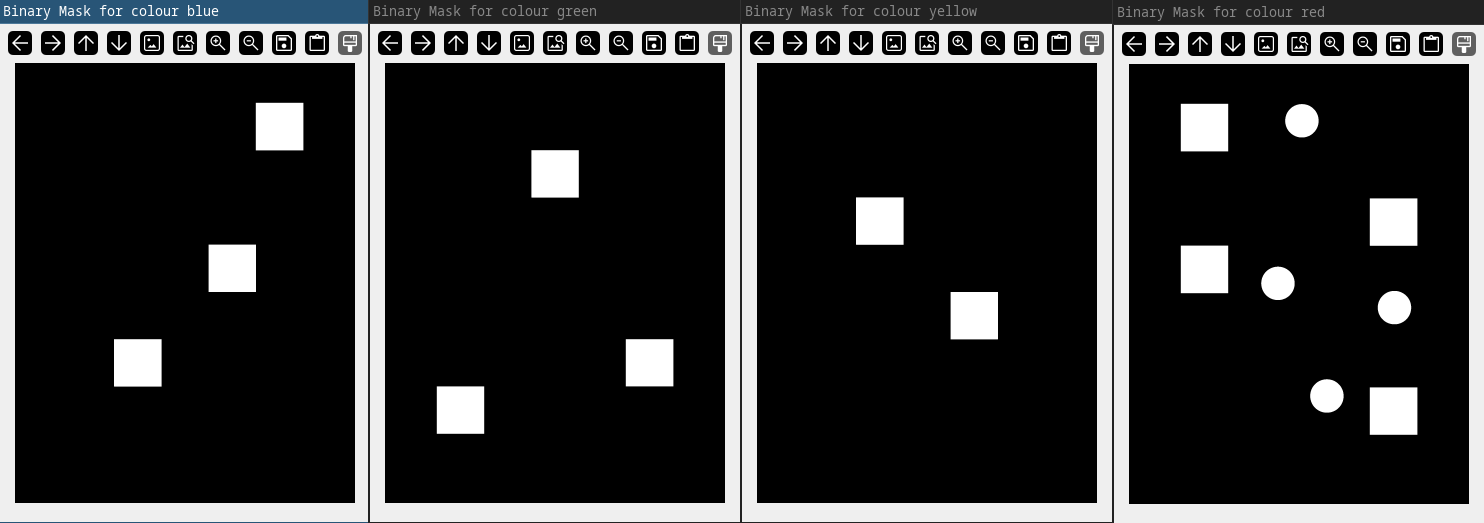
\includegraphics[width=\textwidth]{part_3.png}
    \caption{Binary masks for different colours, using kmeans clustering algorithm to determine regions of different colours.}
    \label{fig:speckled_patterns}
\end{figure} 

\item The circles have circuliartiy about 0.9, while the squares of circularity 0.785. Thus, we set a threshold 0.8 to mark as a circle.
    The images with the bounding boxes around them:
\begin{figure}[htbp]
    \centering
    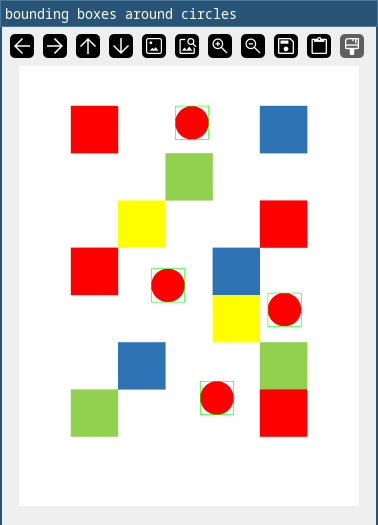
\includegraphics[width=150]{part_4.png}
    \caption{Bounding boxes around circles}
    \label{fig:speckled_patterns}
\end{figure} 

\end{enumerate}


\end{document}
